\documentclass{article}
\usepackage[utf8]{inputenc}
\usepackage{graphicx}
\usepackage{float}
\usepackage{enumerate}
\usepackage{parskip}
\usepackage[numbers, sort]{natbib}
\usepackage{hyperref}
\usepackage{geometry}
 \geometry{
 a4paper,
 total={170mm,257mm},
 left=25mm,
 right=25mm,
 top=30mm,
 bottom=30mm,
 }

\title{Requirements Engineering\\ Conformance checking using activity and trace embeddings}
\author{Group 5 }
\date{December 2020}

\usepackage{natbib}
\usepackage{graphicx}

\begin{document}

\maketitle

\newpage
\tableofcontents
\newpage

% very raw requirements from the meeting
% - the software works correct, i.e. it includes tests
% - similar traces should yield high similarity measurements
% - the software should be able to import a process tree
% - the software should be able to import an event log
% - the software should be able to calculate the trace embeddings and activity with the various methods described in the paper
% - the software can calculate the dissimilarity matrix
% - the software can calculate the fitness and precision as specified
% - the software uses the pm4py library
% - Minimum supported python version 3.7
% - our library should be easy to use
% - the library should have a good documentation
% - The library should use file formats which are consistent with PM4Py
% - The code should be of high quality and good maintainability
% - the software implements different similarity measures, including earth-mover-distance and ICT
% - the software uses an external library for the calculation of the earth-mover-distance
% - the library is designed in a modular way allowing for new embeddings and distance measures to be implemented
% - the software works on recent versions of Linux, Windows and MacOS

\section{Requirements Elicitation and Development}
This phase of requirements engineering begins with identifying stakeholders (various viewpoints) of the system and collecting raw requirements from their point of view. Problems of the raw requirements such as conflicts and lack of details will be resolved after going through requirement analysis. After successful analysis, requirements allocation and flow-down will provide a hierarchical structure of requirements, so that the analyzed requirements can be adequately fulfilled by different specialists of the team.

\subsection{Stakeholders}
Following stakeholders are identified, and their viewpoints will be considered when collecting requirements.
\begin{itemize}
  \item The project team (Chan Yong Lee, Chenyang Li, Denis Razsolkov, Hanbit Chang, Robin Schmitt, Tilman Hoffbauer)
  \item A1 GmbH company (contact person Alessandro Berti)
  \item The user
\end{itemize}

\subsection{Raw Requirements}

\subsubsection{Customer Requirements}
\begin{enumerate}
    \item The software works correctly, i.e. it includes tests
    \item The software uses the PM4Py library
    \item The software should be able to calculate the followings:
    \begin{enumerate}
        \item trace embeddings and activity with the various methods proposed by Peeperkorn et al.\cite{inbook}
        \item dissimilarity matrix
        \item fitness and precision 
    \end{enumerate}
    \item The software implements different similarity measures, such as:
    \begin{enumerate}
        \item Earth Mover's Distance (EMD)
        \item Iterative Constrained Transfers (ICT)
    \end{enumerate}
    \item The software uses an external library for the calculation of the EMD
    \item Similar traces should yield high similarity measurements
    \item The library should be designed in a modular way allowing for new trace embeddings and distance measures to be implemented
    \item The library should have good documentation and be easy to use
\end{enumerate}

\subsubsection{User Requirements}
\begin{enumerate}
    \item The conformance checking service of the program should be precise
    \item The software should provide optimal user experiences/interfaces
    \item The results of the library's calculations should be consistent and should be saved for further analysis
    \item The software should be responsive 
\end{enumerate}

\subsubsection{Developer Requirements}
\begin{enumerate}
    \item The code should be of high quality and good maintainability
    \item The library should use file formats that are consistent with PM4Py
    \begin{enumerate}
        \item The software should be able to import a process tree
        \item The software should be able to import an event log
    \end{enumerate}
\end{enumerate}

\subsubsection{System Requirements}
\begin{enumerate}
  \item The software should work on recent versions of Linux, Windows and \mbox{macOS}.
  \item The software should support python versions from 3.7
\end{enumerate}

\subsection{Requirement Analysis}
After the raw requirements are collected, they have gone through requirement analysis. The viewpoint of the A1 GmbH (especially Alessandro Berti) was intensively considered once more. As a result, the raw requirements are classified into a hierarchical structure, so that implementation workload can be divided adequately to team members throughout the development process, for designing and testing.

\subsection{Allocation and Flow-Down of Requirements}
The result of the requirement analysis in hierarchical structure will be provided in this section. Hierarchically classified requirements will define the interaction between applications and subsystems to fulfill the requirements of the software \cite{inproceedings}.

\subsubsection{High Level}
\begin{description}
\item [H1] The user should be able to configure representation formats (different process models) of the results
\item [H2] The user should be able to compare results of conformance checking
\item [H3] The software should be able to perform conformance checking using methods proposed by Peeperkorn et al.\cite{inbook}
\item [H5] The software should provide a detailed explanation in error cases caused during software execution
\item [H6] The software should provide precise, consistent, and reliable results
\item [H7] The results of the library's calculations should be saved and be able to be recalled for future analysis
\item [H8] The software should support various recent operating systems
\item [H9] The software should be responsive
\item [H10] The software should provide an optimal user experience
\item [H11] The software should consist of clean, maintainable code
\item [H12] The library documentation of the software should provide high readability
\end{description}

\subsubsection{Intermediate Level}
\begin{description}
\item [I1] The software should implement multiple representation formats for the results (\textbf{H1})
\item [I2] Each representation format should be designed for easy interpretation and processing by the user (\textbf{H1, H2, H10, H12})
\item [I3] The software should implement multiple conformance checking methods proposed by Peeperkorn et al.\cite{inbook} (\textbf{H3})
\item [I4] The software should be modular to allow for the addition of new methods in the future (\textbf{H1, H3, H11})
\item [I5] The library should use an easy to understand and consistent error handling technique (\textbf{H5})
\item [I6] There should be an automated test suite for correctness, performance, code style, and platform support (\textbf{H6, H8, H9, H11})
\item [I7] For each representation format there must exist a simple way to persist it. (\textbf{H2, H7})
\item [I8] The software should support Python version $\geq 3.7$ (\textbf{H8})
\item [I9] The software should support \mbox{macOS}, Linux and Windows (\textbf{H8})
\item [I10] All aspects of the software should be well documented (\textbf{H10, H11, H12})
\item [I11] The library should re-use existing software where possible (\textbf{H6, H10, H11})
\item [I12] The library should provide methods for importing a process model and event log. (\textbf{H10})
\end{description}

\subsubsection{Low Level}
\begin{description}
\item [L1] The library should implement the dissimilarity matrix (\textbf{I1, I2, I4})
\item [L2] The library should implement the fitness and precision values (\textbf{I1, I2, I4})
\item [L3] The software should implement the processing step that transforms data into a format that is suited for EMD calculation (\textbf{I3, I4})
\item [L4] The software should implement the processing step that transforms data into a format that is suited for ICT calculation (\textbf{I3, I4})
\item [L5] The library should implement the count of words embedding (\textbf{I3, I4})
\item [L6] The library should implement the Levenshtein distance (\textbf{I3, I4})
\item [L7] The library should use a consistent interface to allow for the addition of future methods for import formats, distance measures, embeddings, and dissimilarity measures (\textbf{I4})
\item [L8] The library should use the Python exception handling technique. (\textbf{I5})
\item [L9] The library should validate its inputs (\textbf{I5})
\item [L10] The test suite should execute unit and integration tests (\textbf{I6})
\item [L11] The test suite should simulate different python versions (\textbf{I6, I8})
\item [L12] The test suite should use a linter to ensure style conformance (\textbf{I6})
\item [L13] The test suite should be executed on different platforms before release (\textbf{I6, I9})
\item [L14] The test suite should check for basic performance measures to ensure responsiveness (\textbf{I6})
\item [L15] The software should allow the dissimilarity matrix to be saved and loaded via NumPy (\textbf{I7})
\item [L16] The software should allow the fitness and precision values to be saved as JSON (\textbf{I7})
\item [L17] There should be an API reference (\textbf{I10})
\item [L18] There should be a user guide (\textbf{I10})
\item [L19] The software should depend on PM4Py \cite{pm4py} (\textbf{I11})
\item [L20] The software should depend on NumPy \cite{numpy} (\textbf{I11})
\item [L21] The software should use an external library for the EMD (\textbf{I11})
\item [L22] The library should be able to import a process tree (\textbf{I12})
\item [L23] The library should be able to import an event log (\textbf{I12})
\end{description}

\section{Functional Model}

Functional models are a useful tool in software development as they can help to visualize processes in a non-technical way. This way, both developers and stakeholders can easily understand the way that the software is supposed to behave.

For our functional model we identified 3 main actors:

\begin{itemize}
    \item The client application: this is the software that the clients will be using and from here, the clients make calls to our library.
    \item Our library: this is the library that we are going to implement and it is split into two sub-components:
    \begin{itemize}
        \item The main module: this is the component that the client application directly communicates with and which returns the dissimilarity matrix and the fitness and precision values. Further, this component makes calls to external libraries and the embedding models to gather all the information that is needed to do the calculations.
        \item The embedding models: this is the component that includes the models that are used to calculate the trace and activity embeddings that are needed to calculate the dissimilarity matrix.
    \end{itemize}
    \item External libraries: this is the library that we are going to use to obtain the playout of the given process model and to calculate the distance measures like the WMD and the ICT.
    
    The model was created using cawemo \cite{cawemo}.
\end{itemize}

\subsection{The model}
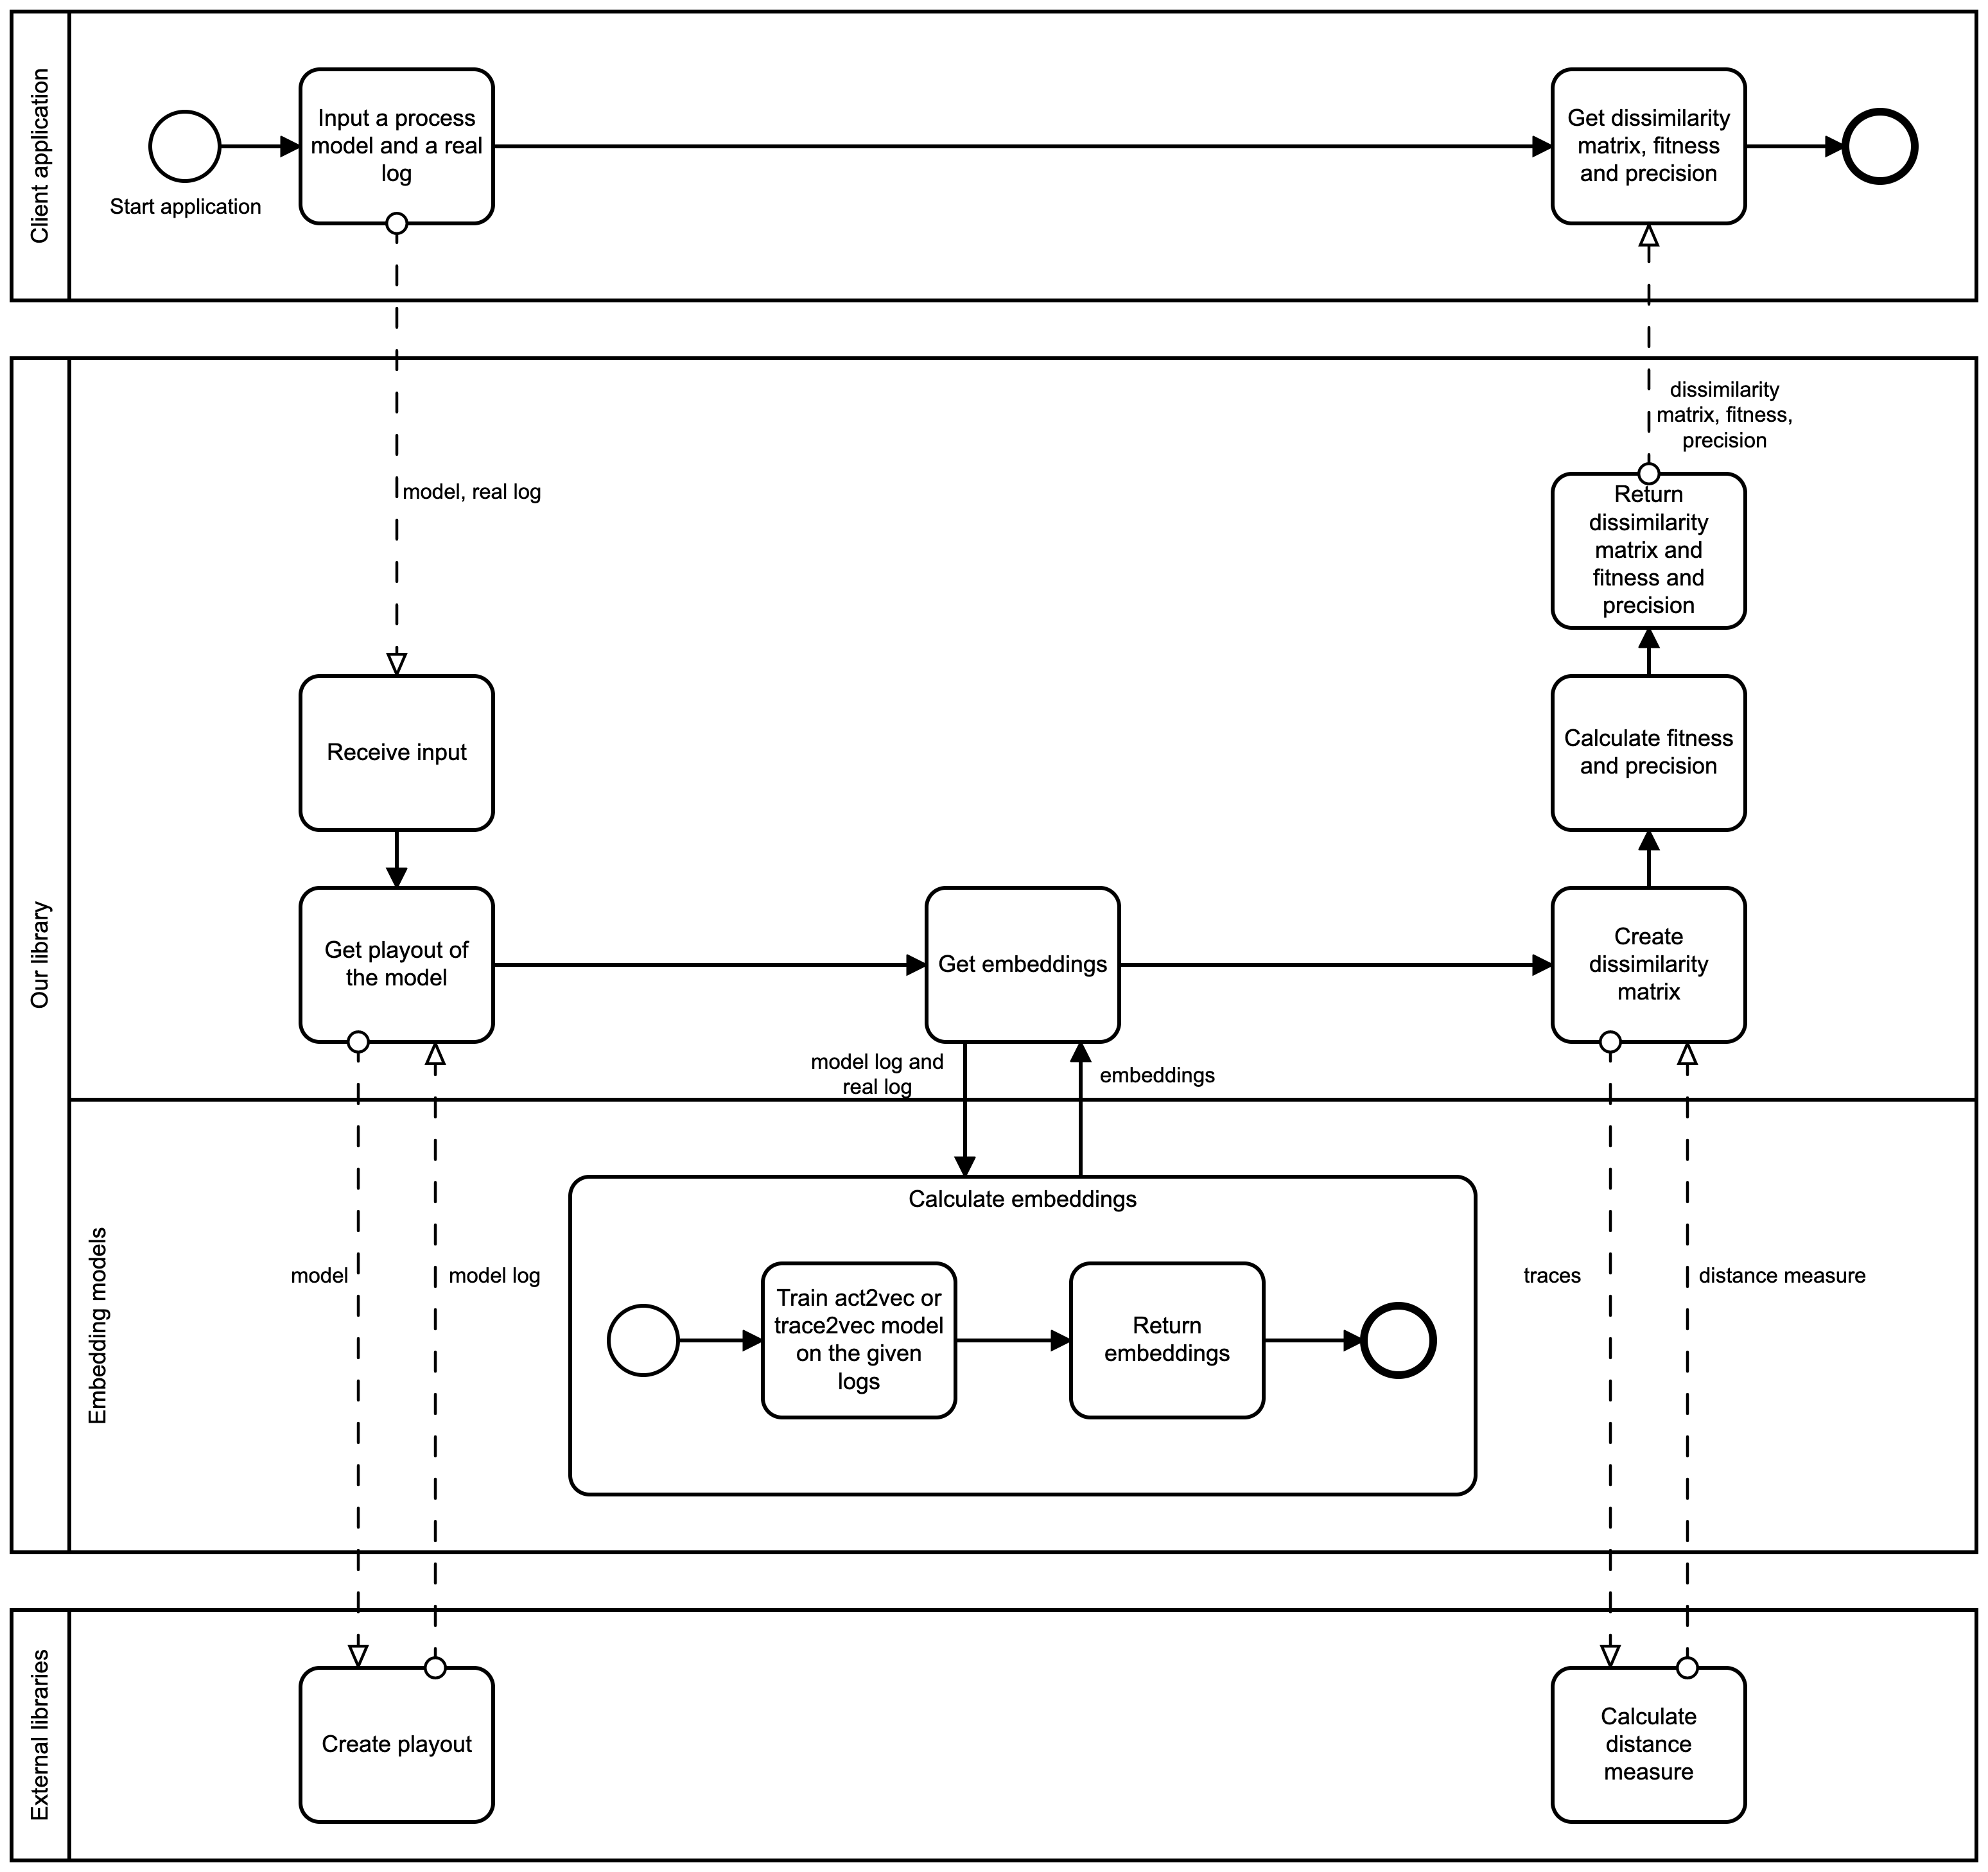
\includegraphics[width=\textwidth]{functional-model.png}

\section{Validation and Verification of Requirements}
To improve the quality of the requirements of the project, it is important different parties involved agree that the requirements are stated correctly. Our team had a meeting with A1 GmbH company (contact person Alessandro Berti) for necessary feedback, so that our requirements meet our user's needs. He pointed out some improvable changes in our requirements and it has been improved as follows:
\begin{enumerate}
    \item [1.]  H5 states about a software error and not an error in the data
    \item [2.] H1 states that our software     supports different types of process-models
    \item [3.] L3 and L4 state that our software does a preprocessing on the data to transform it into suitable input for the calculation of EMD and ICT by an external library
\end{enumerate}

\section{Requirement Management Tools}
Requirements Engineering is a crucial part of a project. It is also a very dynamic part. New requirements can be added, other removed and some can simply have their priority changed. And whilst all of this is happening every member of the team must be up-to-date with the state of the requirements and their assignment. It is easy to see how this can become quite difficult and this is where Requirement Management Tools come in. In this section, we will go over several tools that can help manage requirements with ease.

\subsection{Jama Software}
    Jama Software provides a platform for managing requirements, risk, and tests. This tool is enterprise-grade and enables a team to capture and communicate requirements, progress, goals, and interdependencies. This also has features for reviews, team-collaboration, as well as real-time impact analysis that can be very helpful throughout the entire development process. Another important aspect of Jama Software is the web-based platform, which means that all team members can have an overview of the project from anywhere with a connection to the Internet, without the need for setting anything up on a particular machine.
    
\subsection{Orcanos}
    Orcanos is a requirement managing tool that puts emphasis on visualization and has an intuitive and easy to use interface. This tool offers end-to-end traceability, test management, and simple collaboration tools such as chat and alerts. One interesting feature of this tool is DocGen, which can be very helpful for creating the documentation of the project. Orcanos is highly praised by its user for the quick and helpful support team.
    
\subsection{Caliber}
    Caliber is a tool that offers great features for the visualization of the requirements. It has a simple drag-and-drop interface that makes it easy to use. It allows you to attach images and spreadsheets to requirements and offers impact analysis tools. One major drawback of Caliber is the fact that it does not offer a web-based interface, which means that every team member needs to set it up on their machine.
    
\subsection{Pearls}
    Pearls is an overall useful and affordable requirements management tool that emphasizes collaboration. It offers a multitude of features such as
    notifications about member activity, comments, user role, backlog, specification management, and others. One very useful feature is the ability to create artifacts such as Use Case Document, Requirements Traceability Matrix, Requirements Specification Document, etc. with one click after having defined use cases, actors, conditions, and flows.

\section{Phase review}

\subsection{Chan Yong Lee}
"The requirements engineering phase was obviously a bit more challenging then the project initiation phase. But we, as a team, have completed the given task in a nice problem-solving manner. We first identified what problems we were facing. And then we considered what kind of methods could be employed to solve the problems. As a team, it was not hard to come up with strategies and divided the workload, so that everything could be done with the help of each teammates. I appreciate that everybody was actively participating in the phase, and that everybody was open for feedback from others. I expect that we work in such a good collaborative way in remaining phases of project." 

\subsection{Chenyang Li}
"This phase of the tasks was obviously more difficult than the last one, but our team still managed to get it done on time. Our communication is still smooth and every member have seriously participated in the whole phase. I'm already looking forward to the programming part later on, and I'm sure we as a team will be able to complete the whole course successfully."

\subsection{Denis Razsolkov}
"This phase of the project definitely required more teamwork and management than the last one, but I still think that we did great. Our communication was on point and everyone accomplished their tasks on time, which was essential due to the interdependencies in this particular stage. I am very pleased with our ability to work together and accomplish our goals. I'm definitely looking forward to the next stage of our project, since we will be diving into the coding part of the Praktikum."

\subsection{Hanbit Chang}
"To develop our product with better quality, our team managed to write the document for requirement engineering. With our smooth communication we were able to divide the tasks for each member and accomplish each chapter. I appreciate that everyone participated actively in this project and give his own opinion on others work. In this state, I am confident that our team will do great on next stage of our project and create a high-quality product."

\subsection{Robin Schmitt}

"The biggest challenge of the requirements engineering phase was that the different sections were interdependent, e.g. the functional model could only be created after the requirements of our software were known. Therefore, the coordination of work was even more important than in the first phase. However, we again mastered this challenge by first determining the raw requirements together and then splitting the remaining work so that all the dependencies were fulfilled before starting with a new section. As this phase of development set the structure for our future implementation, I am now excited to see if everything will go as planned."

\subsection{Tilman Hoffbauer}
"The requriements engineering phase is a crucial part of the project, as we define our upcoming work in this phase.
Thus it is of high importance do evaluate the requirements carefully and ensure completeness.
We aimed for completeness by collecting the raw requirements in a group meeting and collecting feedback from our supervisor.
Due to the serial approach in the paper we had high interdependencies between the different chapters in this document, but we managed this with a tight scheduling of internal deadlines, allowing for a good distribution of the work.
I am excited to start coding now where we have planned our work in so much detail!"


\bibliographystyle{plain}
\bibliography{references}
\end{document}
